\subsection{课前提醒模块} % todo subsub

\subsubsection{代码框架及分析}

\subsubsection{课表获取及数据处理原理}

\begin{table}[H]
    \centering
    \begin{tabular}{cc}
        \begin{minipage}[H]{0.4\textwidth}
            \centering
            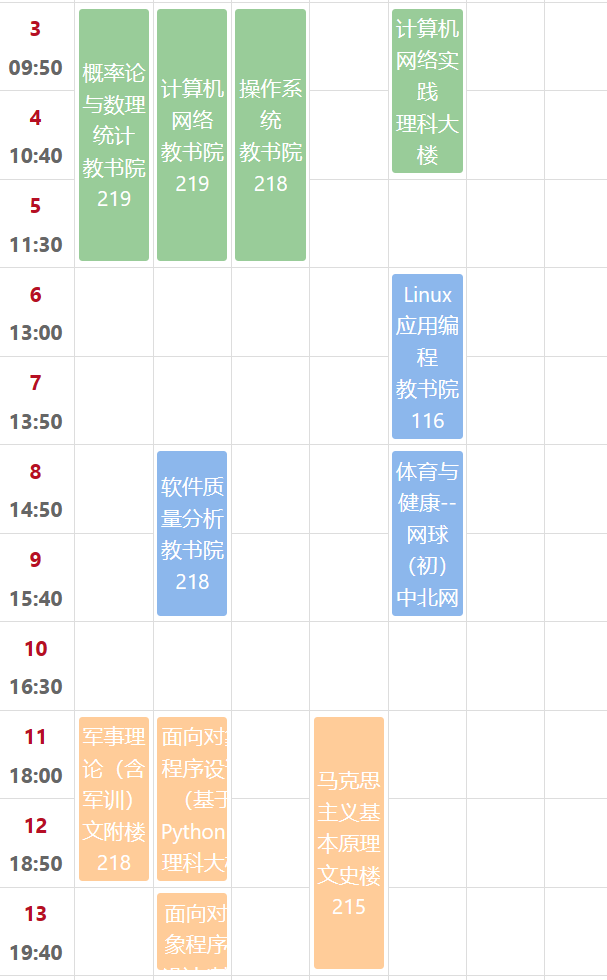
\includegraphics[width=0.5\textwidth]{img/calendar.png}
            \captionof{figure}{ECNU Portal 课表页面}
            \label{fig:login}
        \end{minipage} &
        \begin{minipage}[H]{0.5\textwidth}
            \raggedright
            \begin{rmr}
                进入电脑端 Portal 主页面右侧,我们可以看到自己的课表,使用抓包工具得知,实际上,本课表是存在一个请求 url 的。

                \vspace{0.5cm}

                那么我们通过上述获得的 \texttt{login\_cache},通过 requests 库发起请求,即可实时获取课表。
            \end{rmr}
        \end{minipage}
    \end{tabular}
\end{table}

\begin{figure}[H]
    \centering
    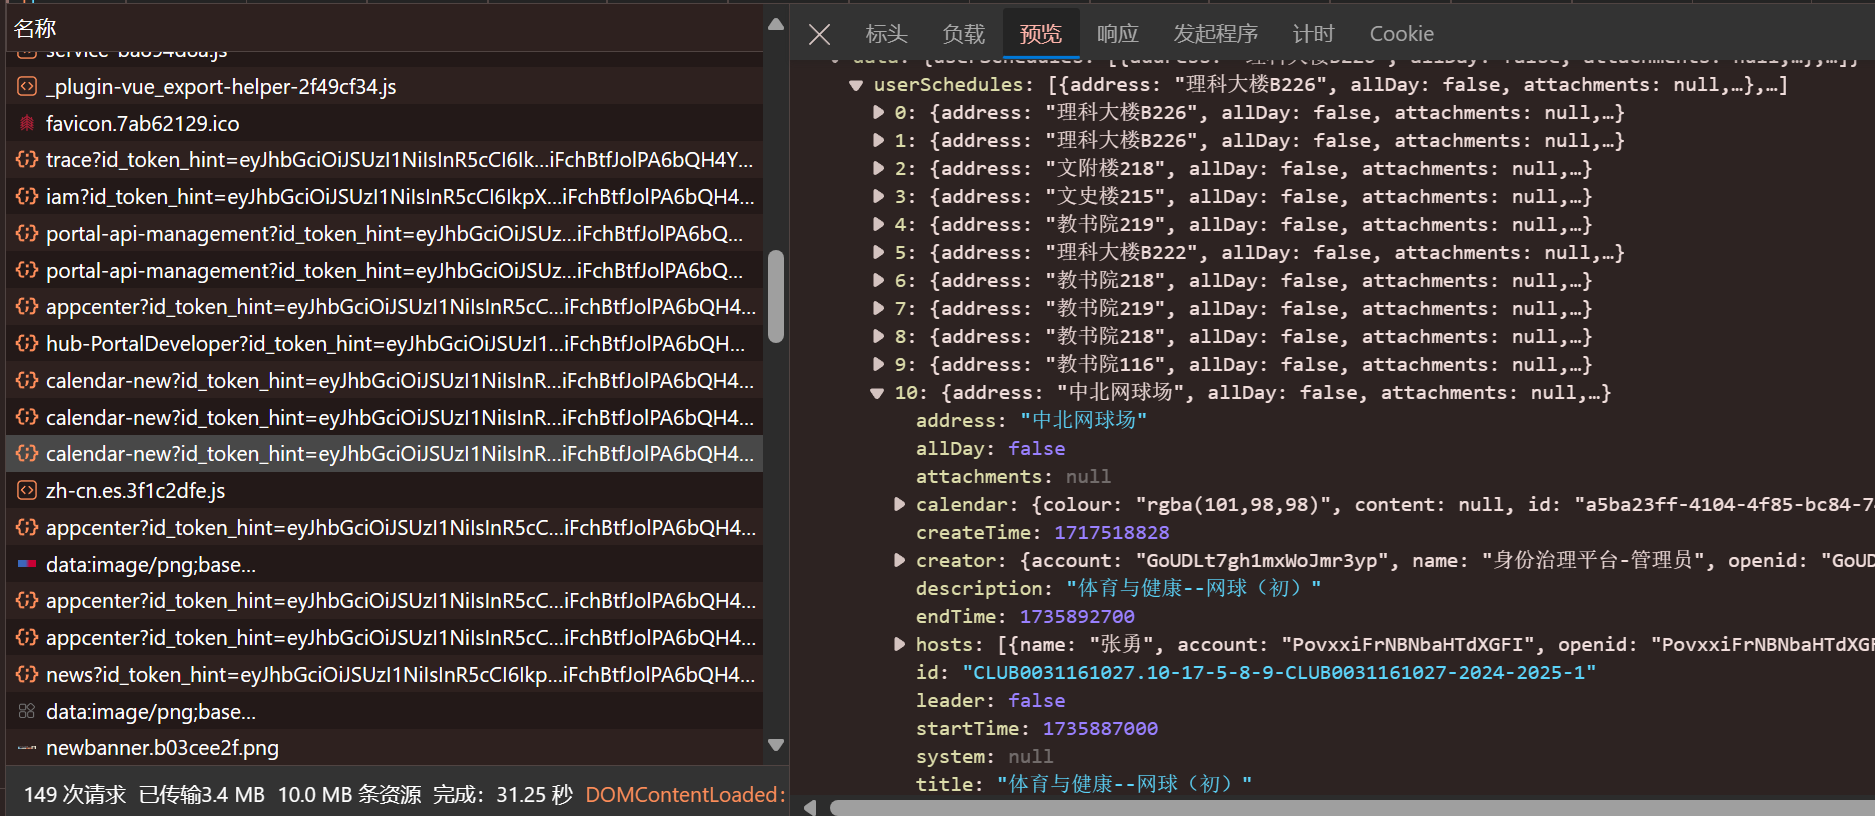
\includegraphics[width=0.8\textwidth]{img/calendar-new-url.png}
    \caption{Portal 课表请求}
    \label{fig:portal_course_table}
\end{figure}

这个 POST 请求采用的是 GraphQL 的查询格式,我们只需要使用 filter 过滤器查询自己所需要的字段即可。

\begin{lstlisting}[language=python]
    USER_SCHEDULES = """
    query ($filter: ScheduleFilter, $userId: String) {
      userSchedules(filter: $filter, userId: $userId) {
        address # 上课地点
        hosts {
          name # 教师名字
        }
        description # 课程信息和描述
        endTime # 结束时间
        startTime # 开始时间
      }
    }
    """
\end{lstlisting}

我们原定的设计是查询当前时刻至次日该时刻,用户的课程安排,如果有课程,上课前的一定时段发送邮件提醒用户去上课。
可以通过插件配置来配置上课前多久提醒用户,相关内容在后面进行详述。

\begin{rmr}
    该功能配置一次后,便可以在后台轮询调用,
    后续我们考虑加入手机端的定位功能,查询用户是否已经到达指定的上课地点,便不发送邮件。
\end{rmr}